\documentclass[a4paper,12pt]{article}
\usepackage{graphicx}
\usepackage{amsmath}
%\usepackage[french]{babel}
%\usepackage[T1]{fontenc}
%%\usepackage[utf8]{inputenc} 

%\frenchspacing

\title{Study of Multimodal Data on Large Data Models for Biomedical Image Analysis}

\begin{document}
\author{Elia Clement Nastasio}
\date{1/3/2024}
\begin{figure}
    
\includegraphics[width=\linewidth]{Imm/polimi_logo.png}
  \end{figure}

\maketitle

\begin{abstract} 
This study wants to analyze the newly developed large data models (LDM) in relation to the analysis of 
biomedical images. In particular how these models change their behaviour when different approaches are 
used when interracting with them.
\end{abstract} 

\tableofcontents

\section{Introduction} 
\section{Large Language Models}
In recent years, the field of natural language processing (NLP) has undergone a remarkable transformation with the 
advent of large language models (LLM). These models have not only overcome the limitations of earlier techniques but 
have also achieved groundbreaking results in both language understanding and generation. Traditional state-of-the-art 
models for sequence prediction problems, such as recurrent neural networks (RNNs), short-long-term-memory or gated RNNs, 
were encumbered by significant computational constraints, with RNNs being notably slow and having restricted access to previous outputs.
A pivotal moment in this evolution occurred in 2017 when Google Brain unveiled the groundbreaking paper 
"Attention Is All You Need," introducing a fundamental element that paved the way for LLN: the transformer.

\subsection{The Transformer Architecture}
The transformer, an innovative architectural paradigm in the domain of natural language processing (NLP), 
represents a milestone that has fundamentally reshaped the landscape of machine comprehension and language generation, 
marking a departure from conventional models. Transformers have introduced pioneering techniques, empowering machines to discern 
intricate linguistic nuances and deliver unparalleled performance across a spectrum of NLP tasks. The next sections will analyze 
each part of the transformers, unraveling how this element is able to generate text in an unseemingly natural manner.
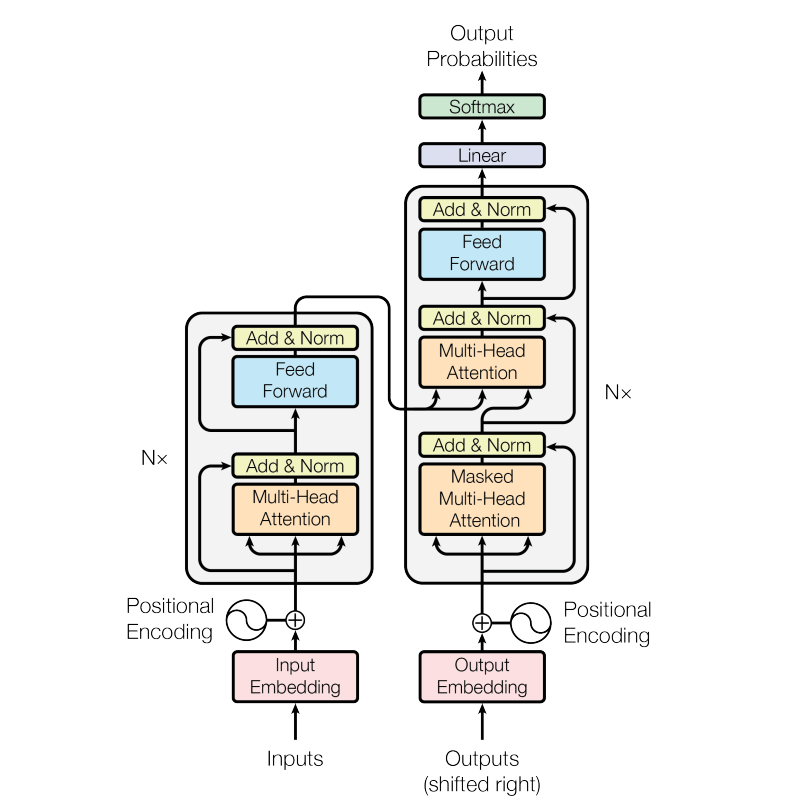
\includegraphics[width=\linewidth]{Imm/transformer_architecture.PNG}

Input Embedding: The initial step involves the tokenization of the input, wherein the input sentence is broken down into smaller tokens,
each assigned a unique Input ID. Various word tokenization methods, such as byte pair encoding and wordpiece tokenization, can be employed.
Some method tokenize whole words while others choose to fragment each sentence into subword tokens. 
A compromise between vocabulary size and flexibility must be made. Each ID is then linked to an embedding, a trainable vector of fixed 
length, denoted as \emph{d\_model}, where \emph{d\_model} = 512 in the paper. The model subsequently adjusts these vectors to more 
accurately represent the meaning of each token. It has been observed that tokens representing similar concept will also have similar 
embedding vectors (e.g. summit and peak). Following word embedding is the critical step of positional encoding. Unlike RNNs or LSTMs, 
the transformer architecture lacks an inherent way of representing the sequential order of words in the input. 
To address this, additional vectors are introduced and summed to the embeddings. Unlike the latter, positional vectors are not 
trainable parameters but are computed only once during model generation. The paper recommends utilizing sine and cosine functions 
to generate the positional encoding, creating patterns in the arrays that convey information about the relative positions between tokens.

\begin{displaymath}
  \begin{align}
    PE_{pos,2i} &= \sin(pos/10000^{2i/d_{model}})
  PE_{pos,2i+1} &= \cos(pos/10000^{2i/d_{model}})
  \end{align} 
\end{displaymath}
The underlying idea is that trigonometric functions generate patterns facilitating the model's understanding of relative token positions. 
This addition aids in capturing the sequential nuances inherent in language. Continuing, we delve into the Multi-head Attention mechanism.
This component is pivotal as it allows the model to consider words located far from the current position, effectively addressing the 
limited scope observed in models like RNNs...

\section{Multimodal Large Language Models}
\section{Conclusions}
\section{References}

\end{document}